% Options for packages loaded elsewhere
\PassOptionsToPackage{unicode}{hyperref}
\PassOptionsToPackage{hyphens}{url}
%
\documentclass[
]{book}
\usepackage{amsmath,amssymb}
\usepackage{lmodern}
\usepackage{iftex}
\ifPDFTeX
  \usepackage[T1]{fontenc}
  \usepackage[utf8]{inputenc}
  \usepackage{textcomp} % provide euro and other symbols
\else % if luatex or xetex
  \usepackage{unicode-math}
  \defaultfontfeatures{Scale=MatchLowercase}
  \defaultfontfeatures[\rmfamily]{Ligatures=TeX,Scale=1}
\fi
% Use upquote if available, for straight quotes in verbatim environments
\IfFileExists{upquote.sty}{\usepackage{upquote}}{}
\IfFileExists{microtype.sty}{% use microtype if available
  \usepackage[]{microtype}
  \UseMicrotypeSet[protrusion]{basicmath} % disable protrusion for tt fonts
}{}
\makeatletter
\@ifundefined{KOMAClassName}{% if non-KOMA class
  \IfFileExists{parskip.sty}{%
    \usepackage{parskip}
  }{% else
    \setlength{\parindent}{0pt}
    \setlength{\parskip}{6pt plus 2pt minus 1pt}}
}{% if KOMA class
  \KOMAoptions{parskip=half}}
\makeatother
\usepackage{xcolor}
\usepackage{color}
\usepackage{fancyvrb}
\newcommand{\VerbBar}{|}
\newcommand{\VERB}{\Verb[commandchars=\\\{\}]}
\DefineVerbatimEnvironment{Highlighting}{Verbatim}{commandchars=\\\{\}}
% Add ',fontsize=\small' for more characters per line
\usepackage{framed}
\definecolor{shadecolor}{RGB}{248,248,248}
\newenvironment{Shaded}{\begin{snugshade}}{\end{snugshade}}
\newcommand{\AlertTok}[1]{\textcolor[rgb]{0.94,0.16,0.16}{#1}}
\newcommand{\AnnotationTok}[1]{\textcolor[rgb]{0.56,0.35,0.01}{\textbf{\textit{#1}}}}
\newcommand{\AttributeTok}[1]{\textcolor[rgb]{0.77,0.63,0.00}{#1}}
\newcommand{\BaseNTok}[1]{\textcolor[rgb]{0.00,0.00,0.81}{#1}}
\newcommand{\BuiltInTok}[1]{#1}
\newcommand{\CharTok}[1]{\textcolor[rgb]{0.31,0.60,0.02}{#1}}
\newcommand{\CommentTok}[1]{\textcolor[rgb]{0.56,0.35,0.01}{\textit{#1}}}
\newcommand{\CommentVarTok}[1]{\textcolor[rgb]{0.56,0.35,0.01}{\textbf{\textit{#1}}}}
\newcommand{\ConstantTok}[1]{\textcolor[rgb]{0.00,0.00,0.00}{#1}}
\newcommand{\ControlFlowTok}[1]{\textcolor[rgb]{0.13,0.29,0.53}{\textbf{#1}}}
\newcommand{\DataTypeTok}[1]{\textcolor[rgb]{0.13,0.29,0.53}{#1}}
\newcommand{\DecValTok}[1]{\textcolor[rgb]{0.00,0.00,0.81}{#1}}
\newcommand{\DocumentationTok}[1]{\textcolor[rgb]{0.56,0.35,0.01}{\textbf{\textit{#1}}}}
\newcommand{\ErrorTok}[1]{\textcolor[rgb]{0.64,0.00,0.00}{\textbf{#1}}}
\newcommand{\ExtensionTok}[1]{#1}
\newcommand{\FloatTok}[1]{\textcolor[rgb]{0.00,0.00,0.81}{#1}}
\newcommand{\FunctionTok}[1]{\textcolor[rgb]{0.00,0.00,0.00}{#1}}
\newcommand{\ImportTok}[1]{#1}
\newcommand{\InformationTok}[1]{\textcolor[rgb]{0.56,0.35,0.01}{\textbf{\textit{#1}}}}
\newcommand{\KeywordTok}[1]{\textcolor[rgb]{0.13,0.29,0.53}{\textbf{#1}}}
\newcommand{\NormalTok}[1]{#1}
\newcommand{\OperatorTok}[1]{\textcolor[rgb]{0.81,0.36,0.00}{\textbf{#1}}}
\newcommand{\OtherTok}[1]{\textcolor[rgb]{0.56,0.35,0.01}{#1}}
\newcommand{\PreprocessorTok}[1]{\textcolor[rgb]{0.56,0.35,0.01}{\textit{#1}}}
\newcommand{\RegionMarkerTok}[1]{#1}
\newcommand{\SpecialCharTok}[1]{\textcolor[rgb]{0.00,0.00,0.00}{#1}}
\newcommand{\SpecialStringTok}[1]{\textcolor[rgb]{0.31,0.60,0.02}{#1}}
\newcommand{\StringTok}[1]{\textcolor[rgb]{0.31,0.60,0.02}{#1}}
\newcommand{\VariableTok}[1]{\textcolor[rgb]{0.00,0.00,0.00}{#1}}
\newcommand{\VerbatimStringTok}[1]{\textcolor[rgb]{0.31,0.60,0.02}{#1}}
\newcommand{\WarningTok}[1]{\textcolor[rgb]{0.56,0.35,0.01}{\textbf{\textit{#1}}}}
\usepackage{longtable,booktabs,array}
\usepackage{calc} % for calculating minipage widths
% Correct order of tables after \paragraph or \subparagraph
\usepackage{etoolbox}
\makeatletter
\patchcmd\longtable{\par}{\if@noskipsec\mbox{}\fi\par}{}{}
\makeatother
% Allow footnotes in longtable head/foot
\IfFileExists{footnotehyper.sty}{\usepackage{footnotehyper}}{\usepackage{footnote}}
\makesavenoteenv{longtable}
\usepackage{graphicx}
\makeatletter
\def\maxwidth{\ifdim\Gin@nat@width>\linewidth\linewidth\else\Gin@nat@width\fi}
\def\maxheight{\ifdim\Gin@nat@height>\textheight\textheight\else\Gin@nat@height\fi}
\makeatother
% Scale images if necessary, so that they will not overflow the page
% margins by default, and it is still possible to overwrite the defaults
% using explicit options in \includegraphics[width, height, ...]{}
\setkeys{Gin}{width=\maxwidth,height=\maxheight,keepaspectratio}
% Set default figure placement to htbp
\makeatletter
\def\fps@figure{htbp}
\makeatother
\setlength{\emergencystretch}{3em} % prevent overfull lines
\providecommand{\tightlist}{%
  \setlength{\itemsep}{0pt}\setlength{\parskip}{0pt}}
\setcounter{secnumdepth}{5}
\usepackage{booktabs}
\ifLuaTeX
  \usepackage{selnolig}  % disable illegal ligatures
\fi
\usepackage[]{natbib}
\bibliographystyle{plainnat}
\IfFileExists{bookmark.sty}{\usepackage{bookmark}}{\usepackage{hyperref}}
\IfFileExists{xurl.sty}{\usepackage{xurl}}{} % add URL line breaks if available
\urlstyle{same} % disable monospaced font for URLs
\hypersetup{
  pdftitle={WGS Shiny Description Document},
  pdfauthor={Tao Chen; Shixue Gou},
  hidelinks,
  pdfcreator={LaTeX via pandoc}}

\title{WGS Shiny Description Document}
\author{Tao Chen; Shixue Gou}
\date{2022-12-08}

\usepackage{amsthm}
\newtheorem{theorem}{Theorem}[chapter]
\newtheorem{lemma}{Lemma}[chapter]
\newtheorem{corollary}{Corollary}[chapter]
\newtheorem{proposition}{Proposition}[chapter]
\newtheorem{conjecture}{Conjecture}[chapter]
\theoremstyle{definition}
\newtheorem{definition}{Definition}[chapter]
\theoremstyle{definition}
\newtheorem{example}{Example}[chapter]
\theoremstyle{definition}
\newtheorem{exercise}{Exercise}[chapter]
\theoremstyle{definition}
\newtheorem{hypothesis}{Hypothesis}[chapter]
\theoremstyle{remark}
\newtheorem*{remark}{Remark}
\newtheorem*{solution}{Solution}
\begin{document}
\maketitle

{
\setcounter{tocdepth}{1}
\tableofcontents
}
\hypertarget{introduction}{%
\chapter{Introduction}\label{introduction}}

\textbf{WGS-Shiny} is a R shiny application that can be easily launched from a local web browser to analyze \emph{whole-genome sequencing} data after variant calling for scientists without programming expertise.

\hypertarget{about}{%
\section{About}\label{about}}

\hypertarget{how-to-start}{%
\section{How to start}\label{how-to-start}}

In this tutorial, we will go through the installation and usage of each module step by step using the example dataset we provided at \emph{github:} \url{https://github.com/123xiaochen/WGS-shiny}.

\hypertarget{requirement}{%
\subsection{Requirement}\label{requirement}}

\begin{enumerate}
\def\labelenumi{\arabic{enumi}.}
\tightlist
\item
  R (\textgreater= 4.2.0)
\item
  Shiny (\textgreater= 1.6.0)
\end{enumerate}

\hypertarget{how-to-install-shiny-packsge}{%
\subsection{How to install shiny packsge}\label{how-to-install-shiny-packsge}}

\begin{enumerate}
\def\labelenumi{\arabic{enumi}.}
\tightlist
\item
  Open \emph{R}.
\item
  User can install the shiny package by the following command in R:
\end{enumerate}

\begin{Shaded}
\begin{Highlighting}[]
\FunctionTok{install.package}\NormalTok{(}\StringTok{"shiny"}\NormalTok{)}
\end{Highlighting}
\end{Shaded}

\hypertarget{how-to-install-and-run-wgs-shiny-locally}{%
\subsection{How to install and run WGS-Shiny locally}\label{how-to-install-and-run-wgs-shiny-locally}}

\begin{enumerate}
\def\labelenumi{\arabic{enumi}.}
\tightlist
\item
  Open \emph{R}.
\item
  Run WGS-Shiny by the following commands in R:
\end{enumerate}

\begin{Shaded}
\begin{Highlighting}[]
\NormalTok{shiny}\SpecialCharTok{::}\FunctionTok{runApp}\NormalTok{(}\StringTok{\textquotesingle{}inst/shiny\textquotesingle{}}\NormalTok{)}
\end{Highlighting}
\end{Shaded}

The first model of WGS-Shiny setting page will pop-up.

\begin{figure}
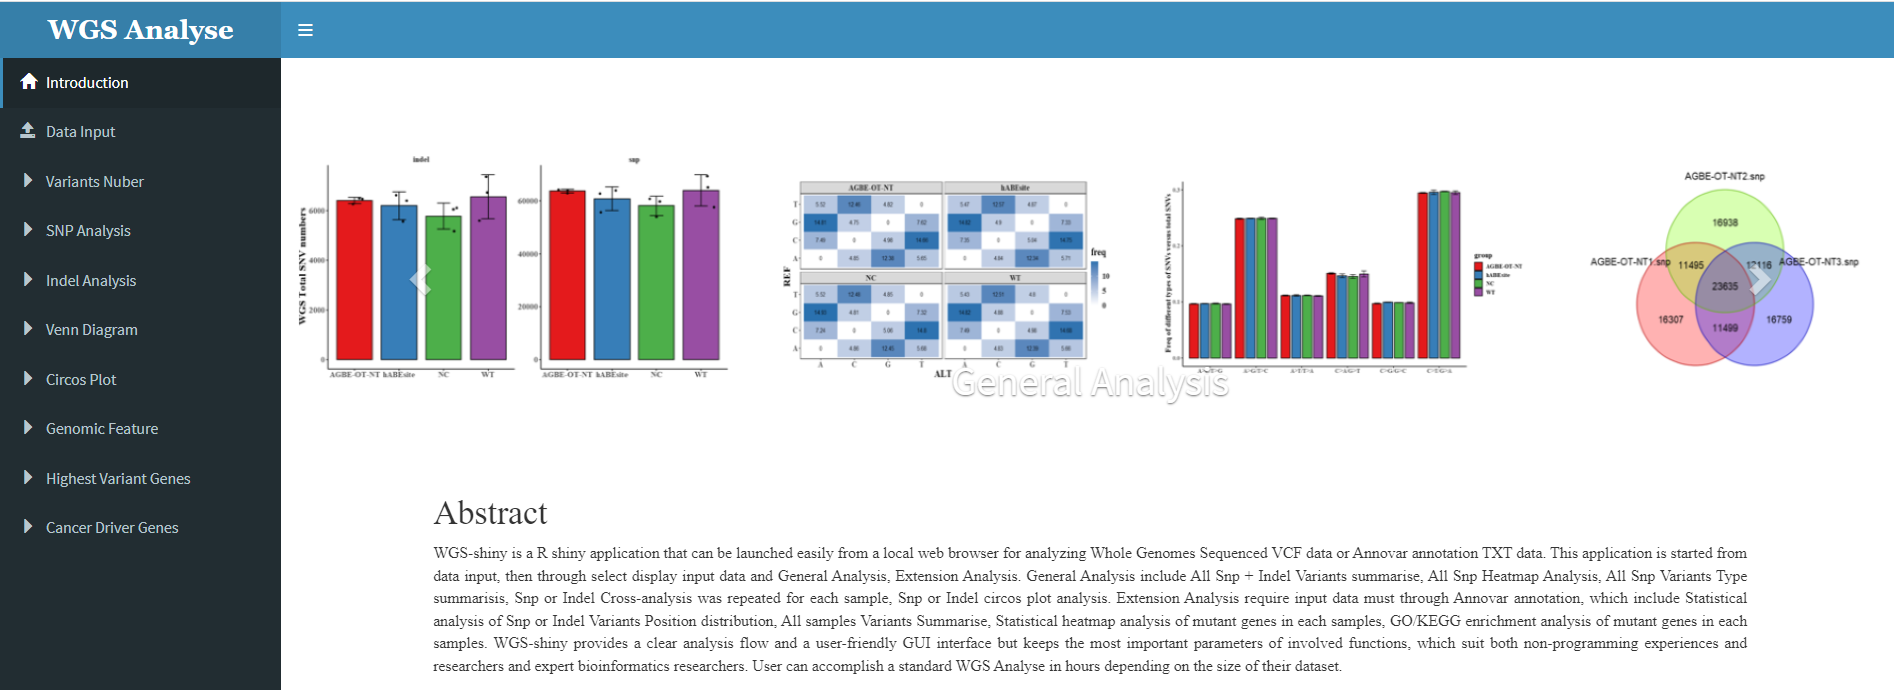
\includegraphics[width=0.8\linewidth]{figure/Main-page} \caption{File-Format}\label{fig:unnamed-chunk-3}
\end{figure}

\hypertarget{prepare-data}{%
\chapter{Prepare data}\label{prepare-data}}

In this Chapter, we will introduce how to prepare two different input data sets:

\hypertarget{source-of-vcf-input-data}{%
\section{Source of VCF input data}\label{source-of-vcf-input-data}}

The Variant Call Format (VCF) is used to record gene sequence variations. It is also the first file format to be understood for genome population correlation analysis. First, the whole genome sequencing file is mapping to the reference, and then the resulting bam file is comprehensively analyzed using variant calling software such as \emph{GATK} and the reference genome data to produce the VCF result.

\hypertarget{source-of-txt-input-data}{%
\section{Source of TXT input data}\label{source-of-txt-input-data}}

TXT files are one of several output formats annotated by \emph{Annovar} (Wang K, Li M, Hakonarson H. 2010), which is able to analyze genetic variations in various genomes using the latest data. Since the input data VCF file of Annovar software only contains the starting position of the mutation, it is necessary to adjust the input data before using, and add the end position of the mutation after the actual position of the mutation. Gene-based annotations reveal variant's direct relationship with known genes and its functional impact, while region-based annotations reveal Variant's relationship with specific segments of different genomes.

\hypertarget{input-data-name-requirements}{%
\section{Input Data name requirements}\label{input-data-name-requirements}}

\hypertarget{input-file-name-requirements}{%
\subsection{Input file name requirements}\label{input-file-name-requirements}}

\begin{figure}
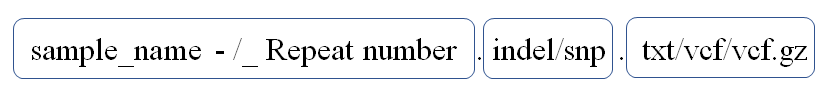
\includegraphics[width=0.8\linewidth]{figure/Input_File_Format} \caption{File-Format}\label{fig:unnamed-chunk-4}
\end{figure}

\begin{enumerate}
\def\labelenumi{\arabic{enumi}.}
\tightlist
\item
  The first box represents the sample name, which can be the group of experiments and the number of repetitions, connected by the character \emph{``-''} or *``\_``*.
\item
  The second box represents the data type, which can be snp or indel data. When snp and indel are not classified in the data, \textbf{this box is not necessary}.
\item
  The third box represents the data format, which can be vcf files, vcf. gz compressed files, and \emph{Annovar} annotated TXT files.
\item
  The contents of the three boxes are connected by \emph{``.''}.
\end{enumerate}

\hypertarget{input-compress-files-requirements}{%
\subsection{Input compress files requirements}\label{input-compress-files-requirements}}

Before uploading the data to WGS-Shiny, that needs to be compressed. The following are the naming requirements for the compressed folder.

\begin{figure}
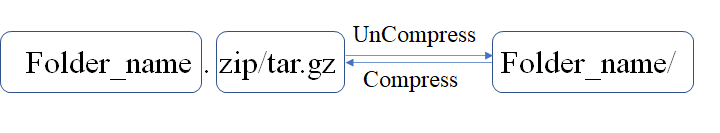
\includegraphics[width=0.8\linewidth]{figure/Fold_Format} \caption{Fold_Format}\label{fig:unnamed-chunk-5}
\end{figure}

\begin{enumerate}
\def\labelenumi{\arabic{enumi}.}
\tightlist
\item
  The compressed file name must be the same as the name of the compressed folder.
\item
  The compressed file can be in \texttt{*.tar.gz} or \texttt{*.zip} format.
\end{enumerate}

\hypertarget{example-data-set-in-wgs-shiny-software}{%
\section{Example data set in WGS-Shiny software}\label{example-data-set-in-wgs-shiny-software}}

We provide a built-in dataset that can be used to explore WGS-Shiny. The data set can be directly loaded into the APP by clicking the button \emph{``Use example data?''} of the data input module (Figure S4-II). The built-in dataset was derived from the sequencing data of published articles, including a control group and three experimental groups, with three replicates in each group (Liang Y, Xie J, Zhang Q, et al.~2022). The sequencing data was first mapping to the reference, followed by gatk Variants calling and Annovar annotations.

\hypertarget{run-the-app}{%
\chapter{Run The App}\label{run-the-app}}

\begin{figure}
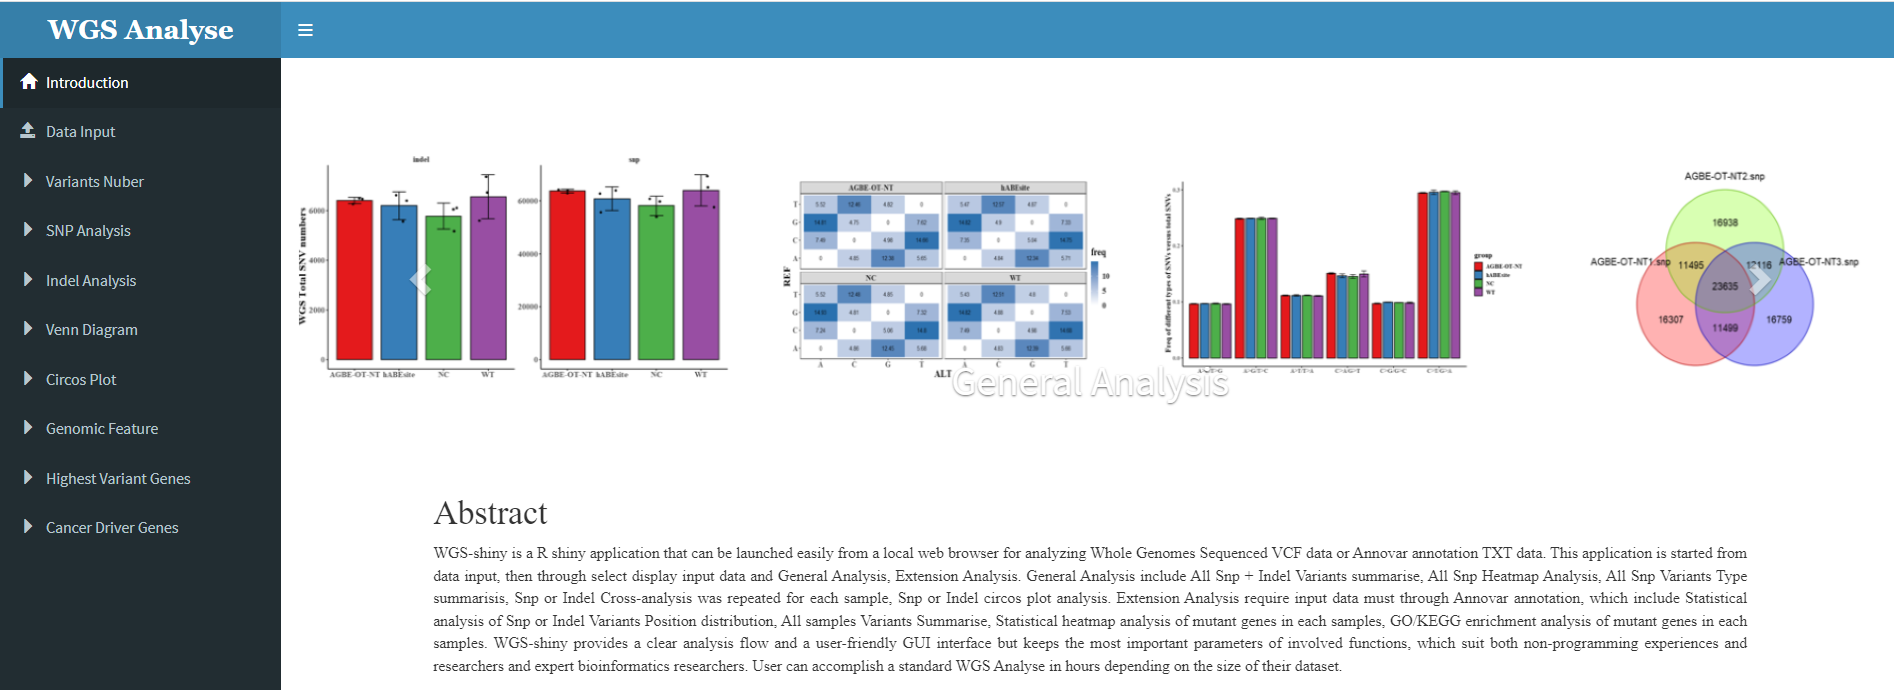
\includegraphics[width=1\linewidth]{figure/Main-page} \caption{Main_Page}\label{fig:unnamed-chunk-6}
\end{figure}

In this Chapter, we will introduce step by step instruction in each module using the example built-in dataset provided at WGS-shiny. After starting the WGS-Shiny , there are a Introduction page and nine modules: (1) Data Input; (2) Variants Numbers; (3) SNP Analysis; (4) Indel Analysis; (5) Venn Diagram; (6) Circos Plot; (7) Genomic Feature; (8) Highest Variants Genes and (9) Cancer Driver Genes on the left panel of WGS-Shiny(Figure S1). For question and bug report, please leave your comment under issue section at github page. Each analysis page includes the analysis method selection module on the left with black background and the analysis module on the right with white background. Click the analysis method in the selection module to enter each analysis page.

\hypertarget{module-1-data-input}{%
\section{Module 1: Data Input}\label{module-1-data-input}}

The purpose of the ``Data Input'' module is for users to input their own data or use the built-in data set. The data reading module consists of three parts: the data selection part on the left, the data display part on the right and the interpretation part of the built-in data below. Add the species selection button (Figure 3.2-I) in the data selection part, load the built-in data button and read the data button (Figure 3.2-II), users can set the button according to their own data (Figure 3.2-III), and there is also a data upload button (Figure 3.2-IV). Sample selection button (Figure 3.2-V) is set in data display section, users can select samples for display.

\begin{figure}
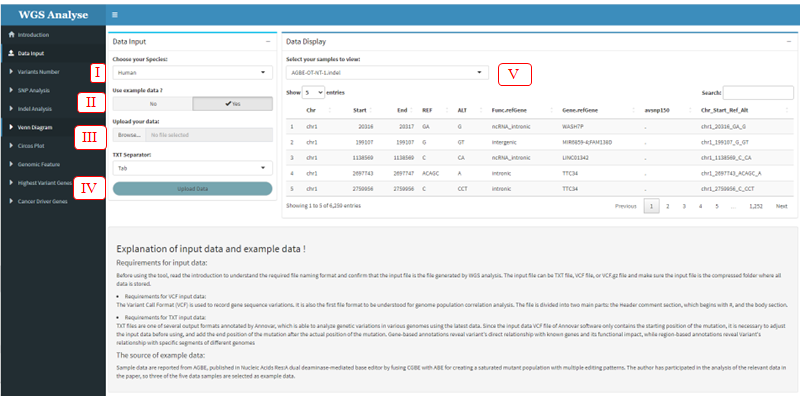
\includegraphics[width=1\linewidth]{figure/Input-page_1} \caption{Data_Input}\label{fig:unnamed-chunk-7}
\end{figure}

\hypertarget{module-2-variants-number}{%
\section{Module 2: Variants Number}\label{module-2-variants-number}}

After uploading the data input, the uploaded input will be automatically divided into SNP and Indel according to the group. The main purpose of the analysis on the second module ``Variants Number'' is to display the number of SNP and Indel.

\begin{figure}
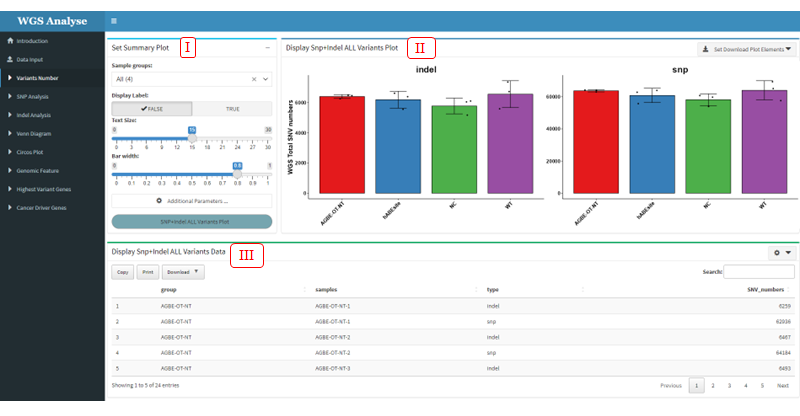
\includegraphics[width=1\linewidth]{figure/1.Variants_numbers_1} \caption{Variants_number}\label{fig:unnamed-chunk-8}
\end{figure}

The analysis module mainly includes three parts. (1) The first part is the selection and setting part, including the selection of data and the setting of graph parameters. At the same time, the transmission command window of ggplot graph command is added to the additional parameters (Figure 3.3-I and Figure 3.4 A-B). (2) The second part is to display the visual results. The drop-down box of the download button is built in the upper right corner of the page, so that users can download the visual results (Figure 3.3-II and Figure 3.4-C). (3) The third part is data display. The upper right corner of this page is built to select the data button, so that users can output the data according to their own needs (Figure 3.4-III and Figure-D).

\begin{figure}
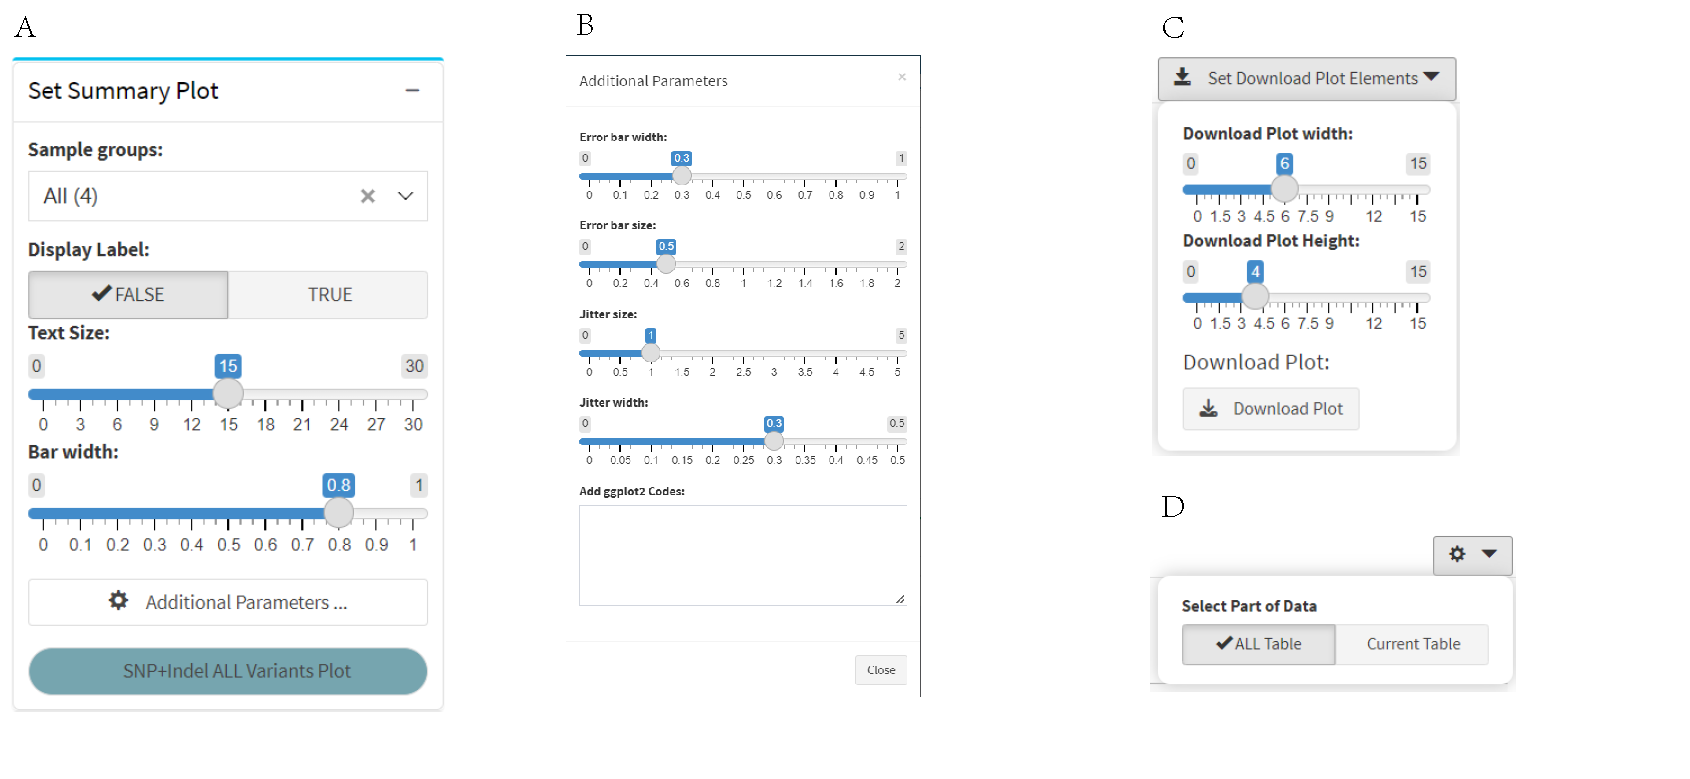
\includegraphics[width=1\linewidth]{figure/1.Variants_numbers_Support} \caption{Variants_number_Elements}\label{fig:unnamed-chunk-9}
\end{figure}

\hypertarget{module-3-snp-analysis}{%
\section{Module 3: SNP Analysis}\label{module-3-snp-analysis}}

This module is to analyze and use heatmap and bar plot to display SNP data of different groups, through which different mutation rates of each group can be clearly seen.

\begin{figure}
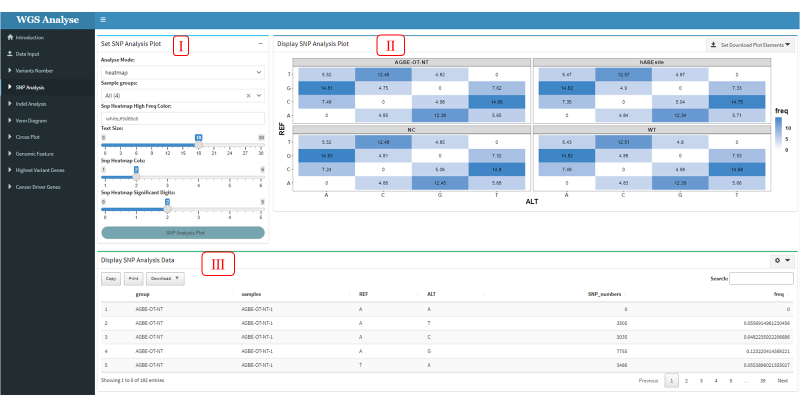
\includegraphics[width=1\linewidth]{figure/2.SNP_Analysis_heatmap_1} \caption{SNP_Analysis_heatmap}\label{fig:unnamed-chunk-10}
\end{figure}

\begin{figure}
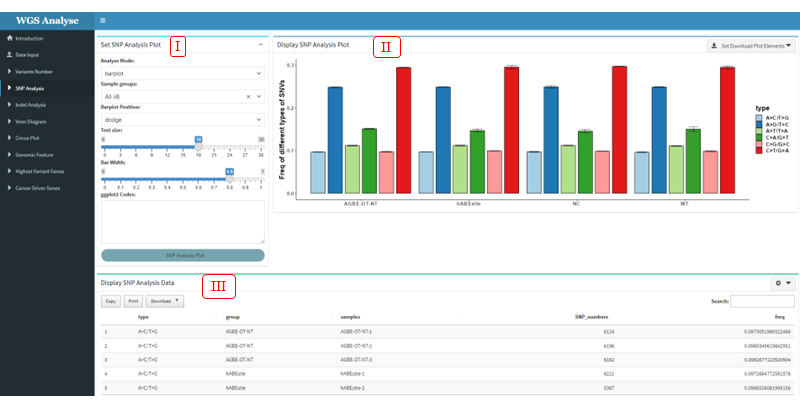
\includegraphics[width=1\linewidth]{figure/2.SNP_Analysis_barplot_1} \caption{SNP_Analysis_Barplot}\label{fig:unnamed-chunk-11}
\end{figure}

This module includes three parts: (1) In the first part ``Set SNP Analysis Plot'', users can choose drawing methods, including heat map and bar chart. The bar chart includes two stacking methods (Figure S3.7), and users can choose interested experimental group and plotting parameters (Figure 3.5-I and Figure 3.6-I). (2) The second part ``Display SNP Analysis Plot'' can display the SNP data use heatmap or bar plot, and user can use download button to download plot (Figure 3.5-II and Figure 3.6-II). (3) The third part ``Display SNP Analysis Data'' can display the heatmap or bar plot data, and also provides the output of the data, the parameters are set the same as in model 2 (Figure 3.5-III and Figure 3.6-III).

\begin{figure}
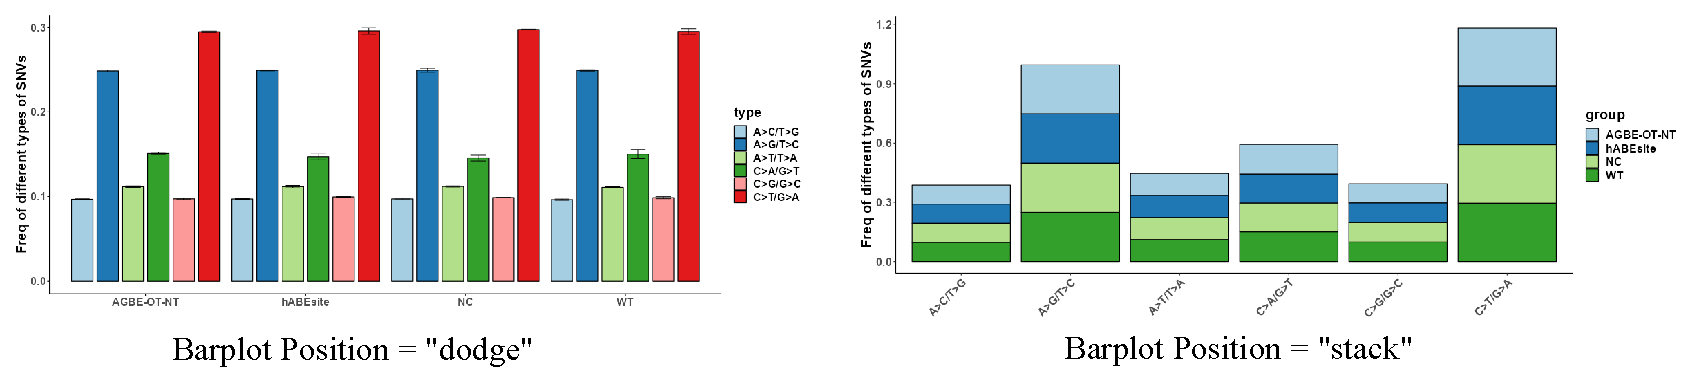
\includegraphics[width=1\linewidth]{figure/2.SNP_Analysis_barplot_ALL_type} \caption{SNP_Analysis_Barpolot_type}\label{fig:unnamed-chunk-12}
\end{figure}

\hypertarget{module-4-indel-analysis}{%
\section{Module 4: Indel Analysis}\label{module-4-indel-analysis}}

This module uses two mapping methods of Indel length density distribution map and Indel length heat map to display Indel data. Through this method, we can intuitively see the situation of various types of mutations in different populations.

\begin{figure}
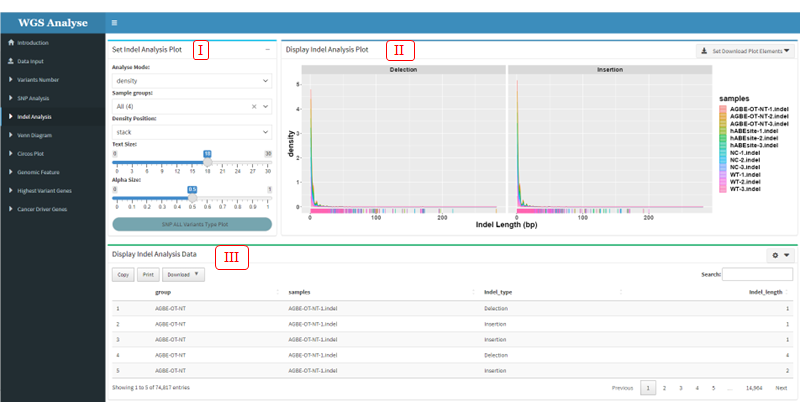
\includegraphics[width=1\linewidth]{figure/3.Indel_Analysis_density_plot_1} \caption{Indel_Analysis_density_plot}\label{fig:unnamed-chunk-13}
\end{figure}

\begin{figure}
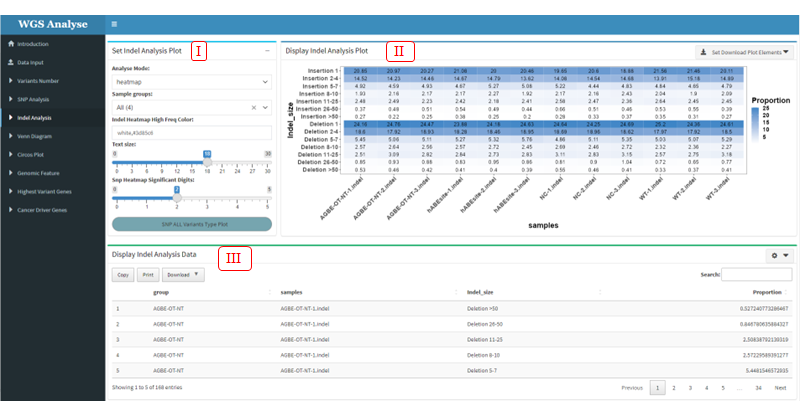
\includegraphics[width=1\linewidth]{figure/3.Indel_Analysis_heatmap_1} \caption{Indel_Analysis_heatmap_plot}\label{fig:unnamed-chunk-14}
\end{figure}

This module consists of three parts: (1) In the first part ``Set Indel Analysis Plot'', users can choose drawing methods, including density plot and heatmap plot (Figure 3.8 and Figure 3.9), in which users can choose interested experimental groups and drawing parameters(Figure 3.8-I and Figure 3.9-I). (2) The second part ``Display Indel Analysis Plot'' can display the Indel data use density plot or heatmap, and user can use download button to download plot (Figure 3.8-II and Figure 3.9-II). (3) The third part ``Display Indel Analysis Data'' can display the density plot or heatmap data, and also provides the output of the data, the parameters are set the same as in model 2 (Figure 3.8-III and Figure 3.9-III).

\hypertarget{module-5-venn-diagram}{%
\section{Module 5: Venn Diagram}\label{module-5-venn-diagram}}

In order to detect the duplicate data credibility of each group, users can cross-analyze the data using the Venn R package (Dusa, Adrian. 2021) and present the visualized results.

\begin{figure}
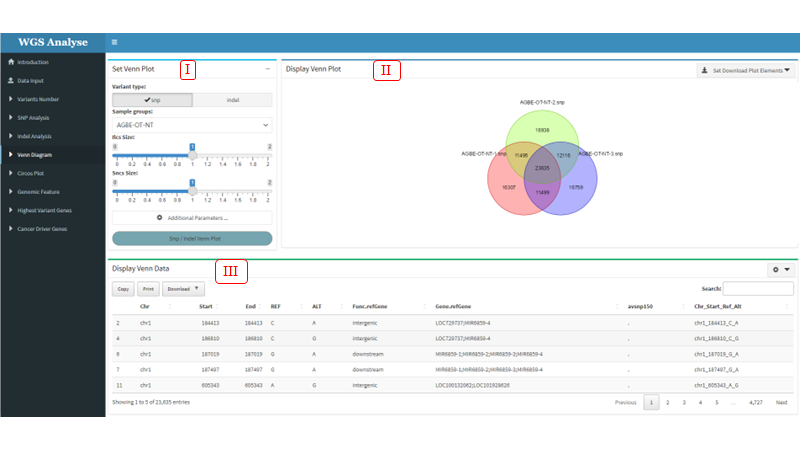
\includegraphics[width=1\linewidth]{figure/4.Venn_Diagram_1} \caption{Venn_Diagram}\label{fig:unnamed-chunk-15}
\end{figure}

The module consists of three parts: (1) The first part can select analysis data and setting visual parameter. Users can select SNP or Indel and interested groups for analysis, and parameters of Venn diagram can be set according to the provided button (Figure 3.10-I). (2) The second part is to visualize the cross data through Venn graph, and download the picture using the download button (Figure 3.10-II). (3) The third part ``Display Venn Data'' shows the cross data and can download the data through the data button, the parameters are set the same as in model 2 (Figure 3.10-III).

\hypertarget{module-6-circos-plot}{%
\section{Module 6: Circos Plot}\label{module-6-circos-plot}}

In order to observe the distribution of SNP or Indel on chromosomes, the ``Circos Plot'' module uses the circlize R package (Gu, Z.et al.~2014) to plot the selected data on a chromosomal circle plot according to the location of mutations.

\begin{figure}
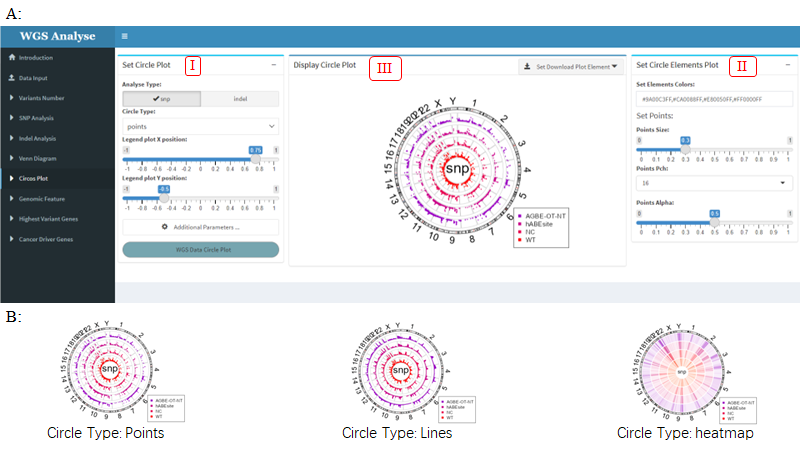
\includegraphics[width=1\linewidth]{figure/5.Circos_plot_1} \caption{Circos_Plot}\label{fig:unnamed-chunk-16}
\end{figure}

This module consists of three parts: (1) The first part is ``Set Circle Plot'', it can select analysis data and setting visual parameter. Users can select SNP or Indel data for analysis. This module sets three display elements, namely point, line and rectangle (Figure 3.11A-I), and can set the position of labels in Circos chart according to the label position button provided. In addition, there are some additional parameters for users to set (Figure 3.11A-II); (2) The second part is ``Set Circle Elements Plot'', which can set the display elements, including the color and size of the elements represented by each group (Figure 3.11B); (3) The third part is ``Display Circle Plot'', which mainly visualizes the data according to the parameter Settings in the previous two steps. Users can use the download button to download the visual results (Figure 3.11A-III).

\hypertarget{module-7-genomic-feature}{%
\section{Module 7: Genomic Feature}\label{module-7-genomic-feature}}

In order to detect the specific position of SNP or Indel in the genome, the ``Genomic Feature'' module makes a statistical analysis of the annotated file according to the genome where the annotated mutation is located, and displays the results with a bar chart.

\begin{figure}
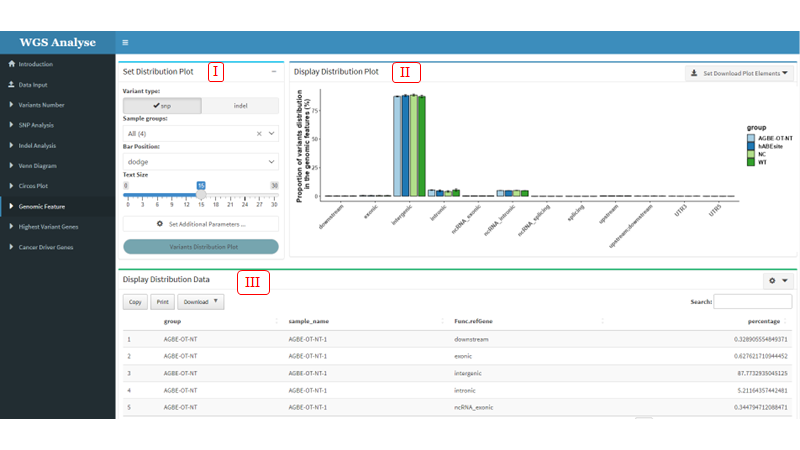
\includegraphics[width=1\linewidth]{figure/6.Genomic_Feature_1} \caption{Genomic_Feature}\label{fig:unnamed-chunk-17}
\end{figure}

This module includes three parts: (1) The first part is ``Set Distribution Plot'', it can select analysis data and setting visual parameter. Users can select SNP or Indel data and interested groups for analysis. The bar chart provides ``stack'' and ``dodge'' stacking modes (Figure 3.13), for users to choose by themselves. Meanwhile, additional parameter Settings are also set in this part, which users can set according to their own needs (Figure 3.12-I); (2) The second part ``Display Distribution Plot'' can display the distribution data use bar plot, and user can use download button to download plot (Figure 3.12-II); (3) The third part ``Display Distribution Data'' can display the bar plot data, and also provides the output of the data, the parameters are set the same as in model 2 (Figure 3.12-III).

\begin{figure}
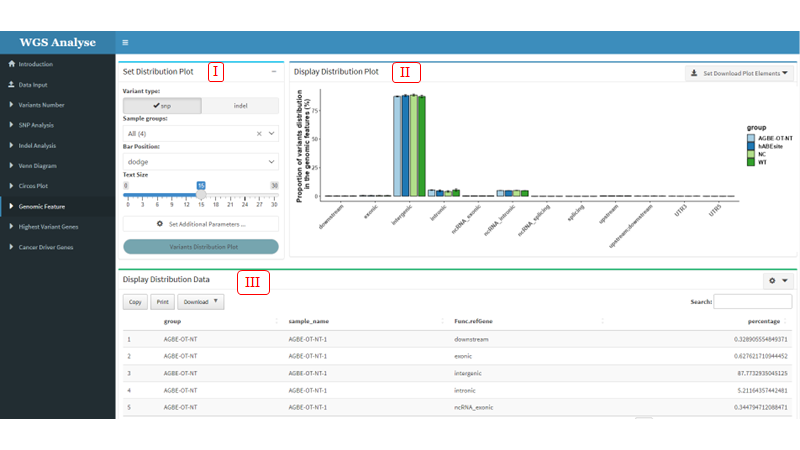
\includegraphics[width=1\linewidth]{figure/6.Genomic_Feature_1} \caption{Genomic_Feature_All_type}\label{fig:unnamed-chunk-18}
\end{figure}

\hypertarget{module-8-highest-variant-genes}{%
\section{Module 8: Highest Variant Genes}\label{module-8-highest-variant-genes}}

In order to visually see the situation of highest mutant genes in each sample, this ``Highest Variant Genes'' module makes statistics on the highest mutant genes in each sample and displays the statistical results.This module includes three parts: (1) The first part ``Set Variants Genes Plot'' is mainly about the selection of data and the setting of visual parameters. Users can select the type of data, the position of mutation on the genome and the sample according to their own needs, and then carry out the next analysis. Meanwhile, additional parameter Settings are also set in this part, which users can set according to their own needs (Figure 3.14-I). (2) The second part ``Display Variants Genes Plot'' can display the Highest mutation data use bar plot, and user can use download button to download plot (Figure 3.14-II). (3) The third part ``Display Variants Genes Data'' can display the bar plot data, and also provides the output of the data, the parameters are set the same as in model 2 (Figure 3.14-III).

\begin{figure}
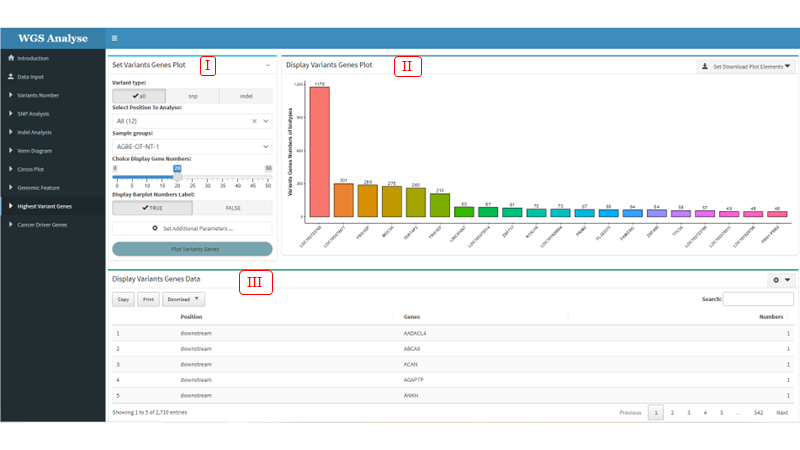
\includegraphics[width=1\linewidth]{figure/7.Highest_Variansts_genes_1} \caption{Highest_Variants_Genes}\label{fig:unnamed-chunk-19}
\end{figure}

\hypertarget{module-9-cancer-driver-genes}{%
\section{Module 9: Cancer Driver Genes}\label{module-9-cancer-driver-genes}}

After the statistics of highly mutated genes in all samples are carried out in Module 8, users can then use this module to select interested samples for heat map comparative analysis and screen out cancer driver genes.This module includes three parts: (1) The first part is mainly about the selection of data and the setting of visual parameters. Users can select the type of data, the position of mutation on the genome and the sample according to their own needs, and then carry out the next analysis. Meanwhile, additional parameter Settings are also set in this part, which users can set according to their own needs (Figure S17-I); (2) The second part can display the different samples Highest mutation data use heatmap, and user can use download button to download plot (Figure S17-II); (3) The third part can display the heatmap data, and also provides the output of the data, the parameters are set the same as in model 2 (Figure S17-III).

\begin{figure}
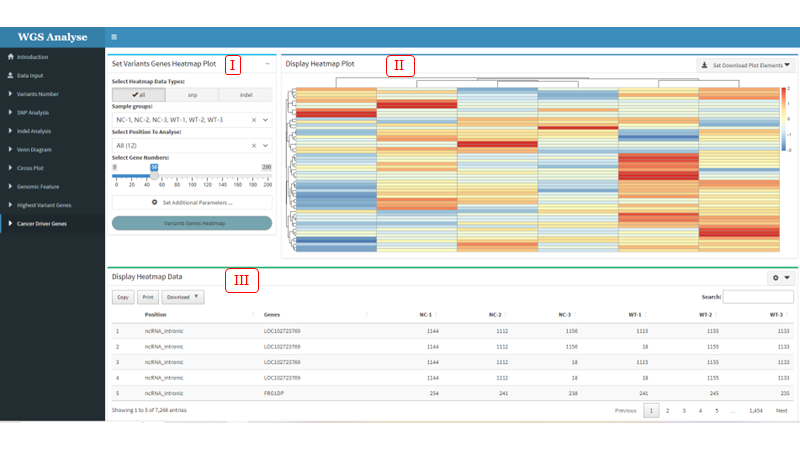
\includegraphics[width=1\linewidth]{figure/8.Cancer_Driver_genes_1} \caption{Cancer_Dirver_Genes}\label{fig:unnamed-chunk-20}
\end{figure}

\hypertarget{parts}{%
\chapter{Parts}\label{parts}}

You can add parts to organize one or more book chapters together. Parts can be inserted at the top of an .Rmd file, before the first-level chapter heading in that same file.

Add a numbered part: \texttt{\#\ (PART)\ Act\ one\ \{-\}} (followed by \texttt{\#\ A\ chapter})

Add an unnumbered part: \texttt{\#\ (PART\textbackslash{}*)\ Act\ one\ \{-\}} (followed by \texttt{\#\ A\ chapter})

Add an appendix as a special kind of un-numbered part: \texttt{\#\ (APPENDIX)\ Other\ stuff\ \{-\}} (followed by \texttt{\#\ A\ chapter}). Chapters in an appendix are prepended with letters instead of numbers.

\hypertarget{footnotes-and-citations}{%
\chapter{Footnotes and citations}\label{footnotes-and-citations}}

\hypertarget{footnotes}{%
\section{Footnotes}\label{footnotes}}

Footnotes are put inside the square brackets after a caret \texttt{\^{}{[}{]}}. Like this one \footnote{This is a footnote.}.

\hypertarget{citations}{%
\section{Citations}\label{citations}}

Reference items in your bibliography file(s) using \texttt{@key}.

For example, we are using the \textbf{bookdown} package \citep{R-bookdown} (check out the last code chunk in index.Rmd to see how this citation key was added) in this sample book, which was built on top of R Markdown and \textbf{knitr} \citep{xie2015} (this citation was added manually in an external file book.bib).
Note that the \texttt{.bib} files need to be listed in the index.Rmd with the YAML \texttt{bibliography} key.

The RStudio Visual Markdown Editor can also make it easier to insert citations: \url{https://rstudio.github.io/visual-markdown-editing/\#/citations}

\hypertarget{blocks}{%
\chapter{Blocks}\label{blocks}}

\hypertarget{equations}{%
\section{Equations}\label{equations}}

Here is an equation.

\begin{equation} 
  f\left(k\right) = \binom{n}{k} p^k\left(1-p\right)^{n-k}
  \label{eq:binom}
\end{equation}

You may refer to using \texttt{\textbackslash{}@ref(eq:binom)}, like see Equation \eqref{eq:binom}.

\hypertarget{theorems-and-proofs}{%
\section{Theorems and proofs}\label{theorems-and-proofs}}

Labeled theorems can be referenced in text using \texttt{\textbackslash{}@ref(thm:tri)}, for example, check out this smart theorem \ref{thm:tri}.

\begin{theorem}
\protect\hypertarget{thm:tri}{}\label{thm:tri}For a right triangle, if \(c\) denotes the \emph{length} of the hypotenuse
and \(a\) and \(b\) denote the lengths of the \textbf{other} two sides, we have
\[a^2 + b^2 = c^2\]
\end{theorem}

Read more here \url{https://bookdown.org/yihui/bookdown/markdown-extensions-by-bookdown.html}.

\hypertarget{callout-blocks}{%
\section{Callout blocks}\label{callout-blocks}}

The R Markdown Cookbook provides more help on how to use custom blocks to design your own callouts: \url{https://bookdown.org/yihui/rmarkdown-cookbook/custom-blocks.html}

\hypertarget{sharing-your-book}{%
\chapter{Sharing your book}\label{sharing-your-book}}

\hypertarget{publishing}{%
\section{Publishing}\label{publishing}}

HTML books can be published online, see: \url{https://bookdown.org/yihui/bookdown/publishing.html}

\hypertarget{pages}{%
\section{404 pages}\label{pages}}

By default, users will be directed to a 404 page if they try to access a webpage that cannot be found. If you'd like to customize your 404 page instead of using the default, you may add either a \texttt{\_404.Rmd} or \texttt{\_404.md} file to your project root and use code and/or Markdown syntax.

\hypertarget{metadata-for-sharing}{%
\section{Metadata for sharing}\label{metadata-for-sharing}}

Bookdown HTML books will provide HTML metadata for social sharing on platforms like Twitter, Facebook, and LinkedIn, using information you provide in the \texttt{index.Rmd} YAML. To setup, set the \texttt{url} for your book and the path to your \texttt{cover-image} file. Your book's \texttt{title} and \texttt{description} are also used.

This \texttt{gitbook} uses the same social sharing data across all chapters in your book- all links shared will look the same.

Specify your book's source repository on GitHub using the \texttt{edit} key under the configuration options in the \texttt{\_output.yml} file, which allows users to suggest an edit by linking to a chapter's source file.

Read more about the features of this output format here:

\url{https://pkgs.rstudio.com/bookdown/reference/gitbook.html}

Or use:

\begin{Shaded}
\begin{Highlighting}[]
\NormalTok{?bookdown}\SpecialCharTok{::}\NormalTok{gitbook}
\end{Highlighting}
\end{Shaded}


  \bibliography{book.bib,packages.bib}

\end{document}
